\iffalse
\let\negmedspace\undefined
\let\negthickspace\undefined
\documentclass[journal,12pt,twocolumn]{IEEEtran}
\usepackage{cite}
\usepackage{amsmath,amssymb,amsfonts,amsthm}
\usepackage{algorithmic}
\usepackage{graphicx}
\usepackage{textcomp}
\usepackage{xcolor}
\usepackage{txfonts}
\usepackage{listings}
\usepackage{enumitem}
\usepackage{mathtools}
\usepackage{gensymb}
\usepackage{comment}
\usepackage[breaklinks=true]{hyperref}
\usepackage{tkz-euclide} 
\usepackage{listings}
\usepackage{gvv}                                        
\def\inputGnumericTable{}                                 
\usepackage[latin1]{inputenc}                                
\usepackage{color}                                            
\usepackage{array}                                            
\usepackage{longtable}                                       
\usepackage{calc}                                             
\usepackage{multirow}                                         
\usepackage{hhline}                                           
\usepackage{ifthen}                                           
\usepackage{lscape}
\newtheorem{theorem}{Theorem}[section]
\newtheorem{problem}{Problem}
\newtheorem{proposition}{Proposition}[section]
\newtheorem{lemma}{Lemma}[section]
\newtheorem{corollary}[theorem]{Corollary}
\newtheorem{example}{Example}[section]
\newtheorem{definition}[problem]{Definition}
\newcommand{\BEQA}{\begin{eqnarray}}
\newcommand{\EEQA}{\end{eqnarray}}
\newcommand{\define}{\stackrel{\triangle}{=}}
\theoremstyle{remark}
\newtheorem{rem}{Remark}
\begin{document}

\bibliographystyle{IEEEtran}
\vspace{3cm}

\title{DISCRETE}
\author{EE23BTECH11006 - Ameen Aazam$^{*}$% <-this % stops a space
}
\maketitle
\newpage
\bigskip

\renewcommand{\thefigure}{\theenumi}
\renewcommand{\thetable}{\theenumi}

\vspace{3cm}
\textbf{Question :}
Consider a carrier signal which is amplitude modulated by a single-tone sinusoidal message signal with a modulation index of $50\%$. If the carrier and one of the sidebands are suppressed in the modulated signal, the percentage of power saved (rounded off to one decimal place) is \ldots.

\hfill(GATE EC 2021)

\solution
\fi
\begin{table}[htbp]
    \centering
    \begin{tabular}{|c|c|c|} \hline
      \textbf{Parameters} & \textbf{Values} & \textbf{Description} \\ \hline
      $m$ & $50\%$ & Percentage modulation \\ \hline
      $x_c\brak{t}$ & & Carrier signal \\ \hline
      $f_c\brak{t}$ & $1000 Hz$ & Carrier signal frequency \\ \hline
      $x_m\brak{t}$ & & Message signal \\ \hline
      $f_m\brak{t}$ & $25 Hz$ & Message signal frequency \\ \hline
      $A_c$ & & Amplitude of Carrier signal \\ \hline
      $P_t$ & & Total power of the modulated AP \\ \hline
      $P_c$ & $\frac{A_c^2}{2}$ & Power of the carrier signal \\ \hline
      $P_s$ & & Saved power \\ \hline
    \end{tabular}
    \vspace{3pt}
    \caption{Parameters}
\end{table}

The percentage modulation,
\begin{align}
    m=50\%=0.5
\end{align}
Suppose, we have the carrier signal as,
\begin{align}
    x_c\brak{t}=A_c\sin{\brak{2\pi f_ct}}
\end{align}
So the message signal,
\begin{align}
    x_m\brak{t}=mA_c\sin{\brak{2\pi f_mt}}
\end{align}
And the modulated signal,
\begin{align}
    y\brak{t}=A_c\brak{1+m\sin{\brak{2\pi f_mt}}}\sin{\brak{2\pi f_ct}}
\end{align}
Now the modulated signal in the frequency domain looks like,
\begin{figure}[h!]
    \centering
    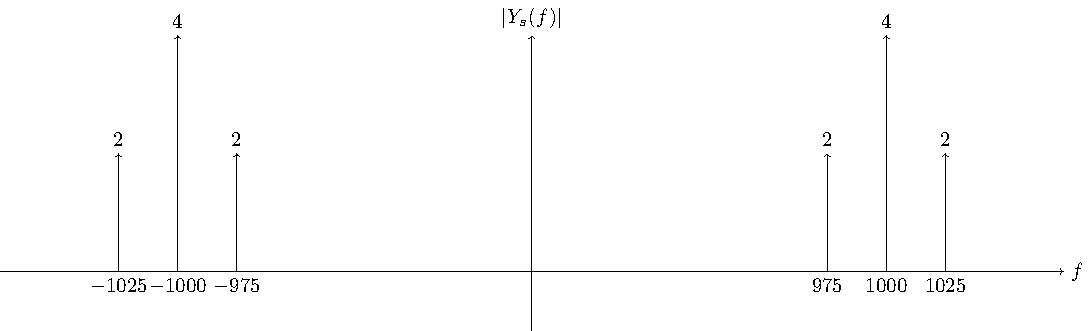
\includegraphics[width=\columnwidth]{2021/EC/22/figs/modulated.pdf}
    \caption{Modulated Signal}
\end{figure}
After the carrier signal and one of the side bands are removed,
\begin{figure}[h!]
    \centering
    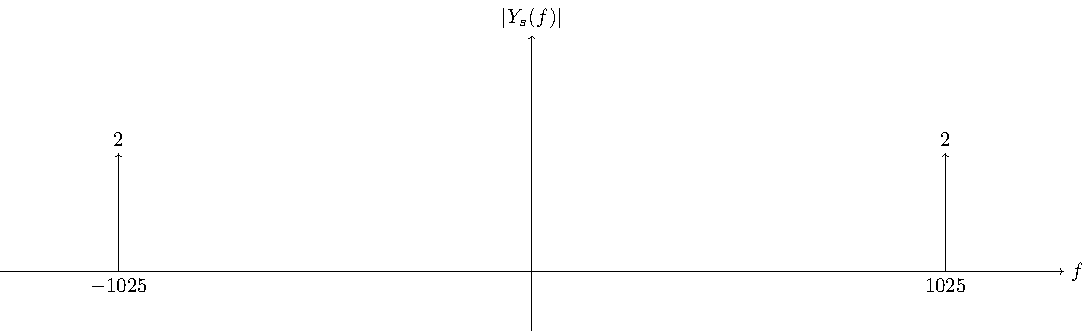
\includegraphics[width=\columnwidth]{2021/EC/22/figs/suppressed.pdf}
    \caption{Suppressed Signal}
\end{figure}
The total power is due to the carrier and the two sidebands,
\begin{align}
    P_t=P_c\sbrak{1+\frac{m^2}{2}}
\end{align}
Now as the carrier signal and one of the sidebands are suppressed then total saved power,
\begin{align}
    P_s=P_c\sbrak{1+\frac{m^2}{4}}
\end{align}
So percentage power saved,
\begin{align}
    &=\frac{P_s}{P_t}\times100\% \\
    &=\frac{P_c\sbrak{1+\frac{m^2}{4}}}{P_c\sbrak{1+\frac{m^2}{2}}}\times100\% \\
    &=\frac{1+\frac{1}{16}}{1+\frac{1}{8}}\times100\% \\
    &=94.44\%
\end{align}
Hence, the percentage power saved is $94.4\%$.
%\end{document}
